\chapter{Figuras dos reservatórios} \label{ch:figurasReservatorios}

Aqui estão apresentadas os grids dos casos C, D e E que foram utilizados para a exposição dos resultados.
As escalas dos casos D e E foram omitidas por se tratarem de modelos reais e os dados, portanto, são sensíveis para a Petrobras.



\begin{figure}[ht]
\center
\subfigure[ ]{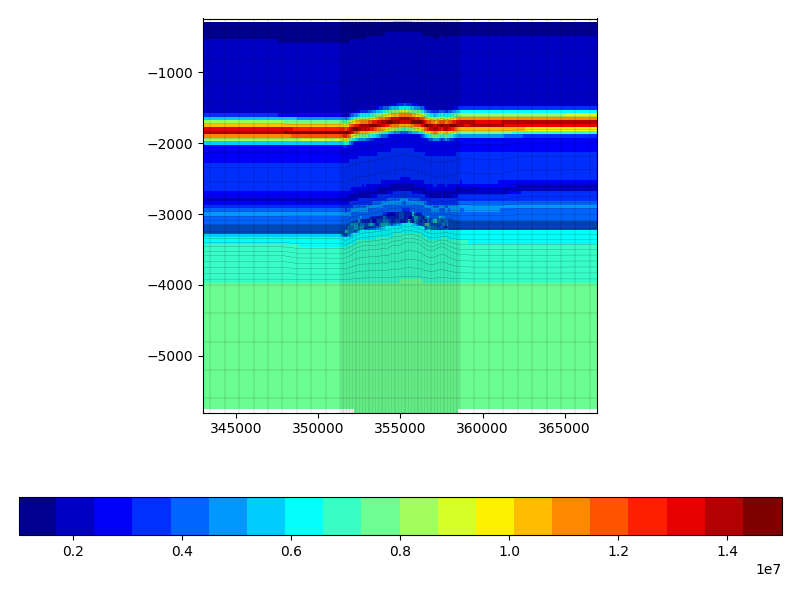
\includegraphics[width=0.45\textwidth]{append/figs/pituba_young.png}}
\qquad
\subfigure[ ]{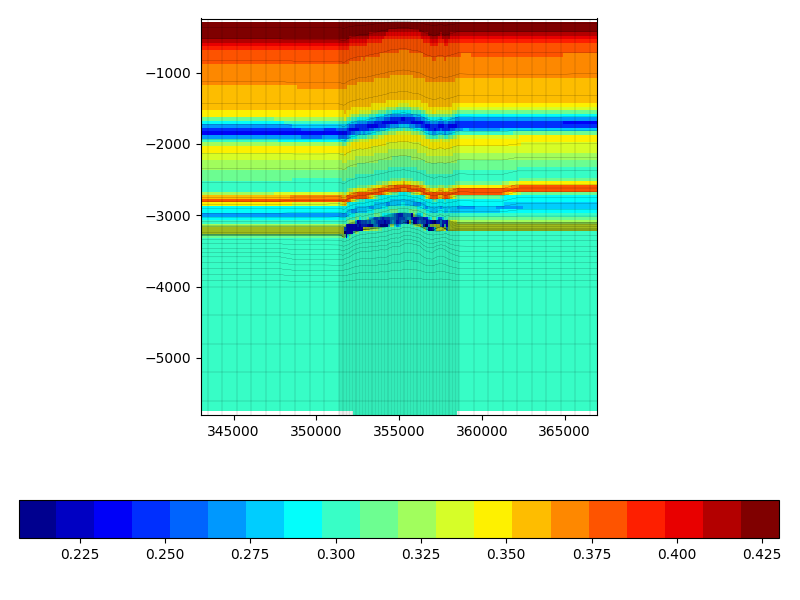
\includegraphics[width=0.45\textwidth]{append/figs/pituba_poisson.png}}
\caption{Propriedades módulo de Young (a) e coeficiente de poisson (b) para caso C } \label{fig:casoCgrid}
\end{figure}

\begin{figure}[ht]

\center
\subfigure[ ]{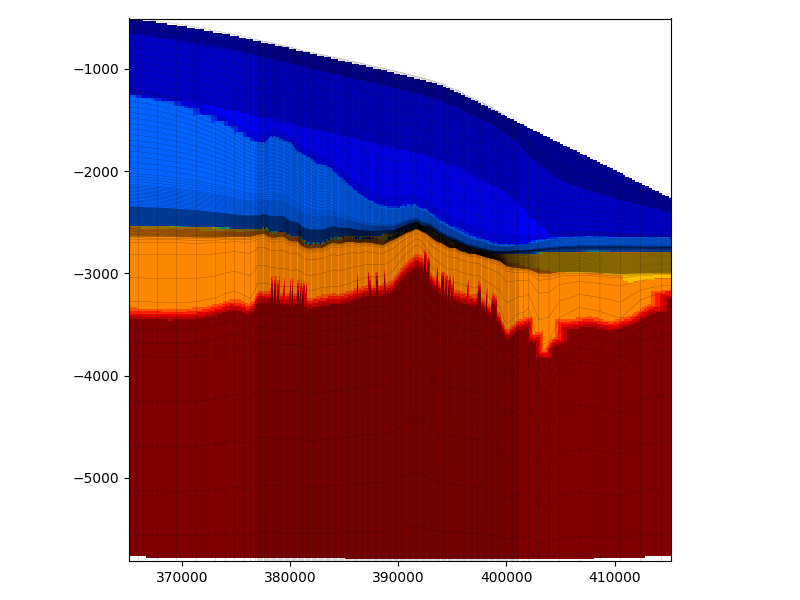
\includegraphics[width=\textwidth]{append/figs/refined_young.png}}
\qquad
\subfigure[ ]{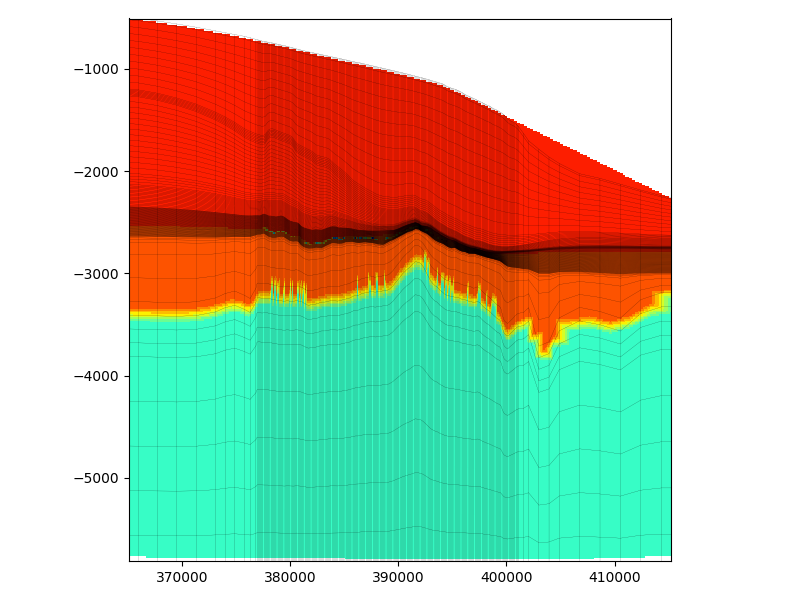
\includegraphics[width=\textwidth]{append/figs/refined_poisson.png}}
\caption{Propriedades módulo de Young (a) e coeficiente de poisson (b) para caso D } \label{fig:casoDgrid}
\end{figure}


\begin{figure}[h]
\center
\subfigure[ ]{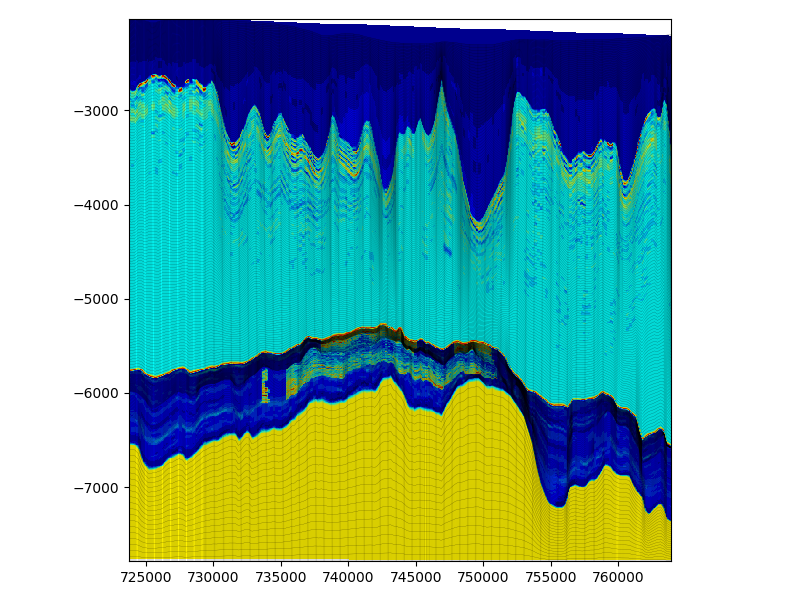
\includegraphics[width=\textwidth]{append/figs/93MM_young.png}}
\qquad
    \subfigure[ ]{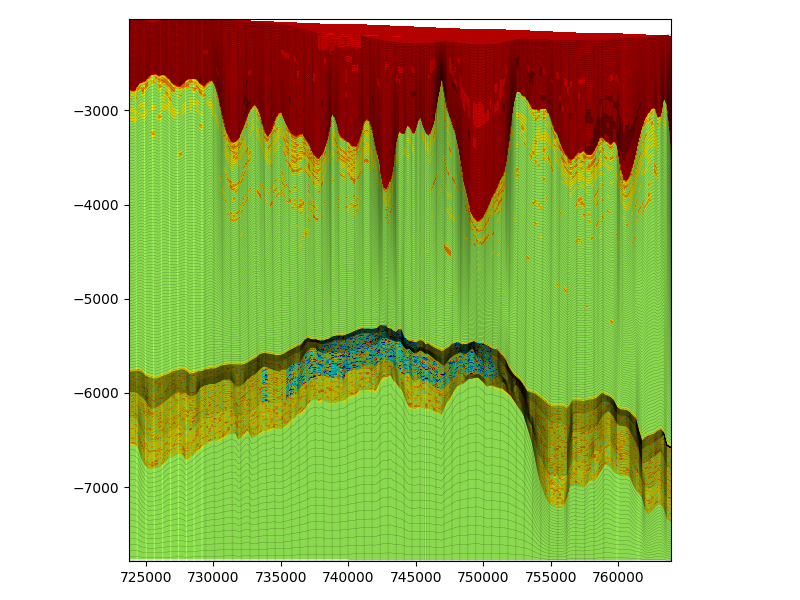
\includegraphics[width=\textwidth]{append/figs/93MM_poisson.png}}
\caption{Propriedades módulo de Young (a) e coeficiente de poisson (b) para caso E } \label{fig:casoEgrid}
\end{figure}


\begin{figure}[h]
\center
\subfigure[ ]{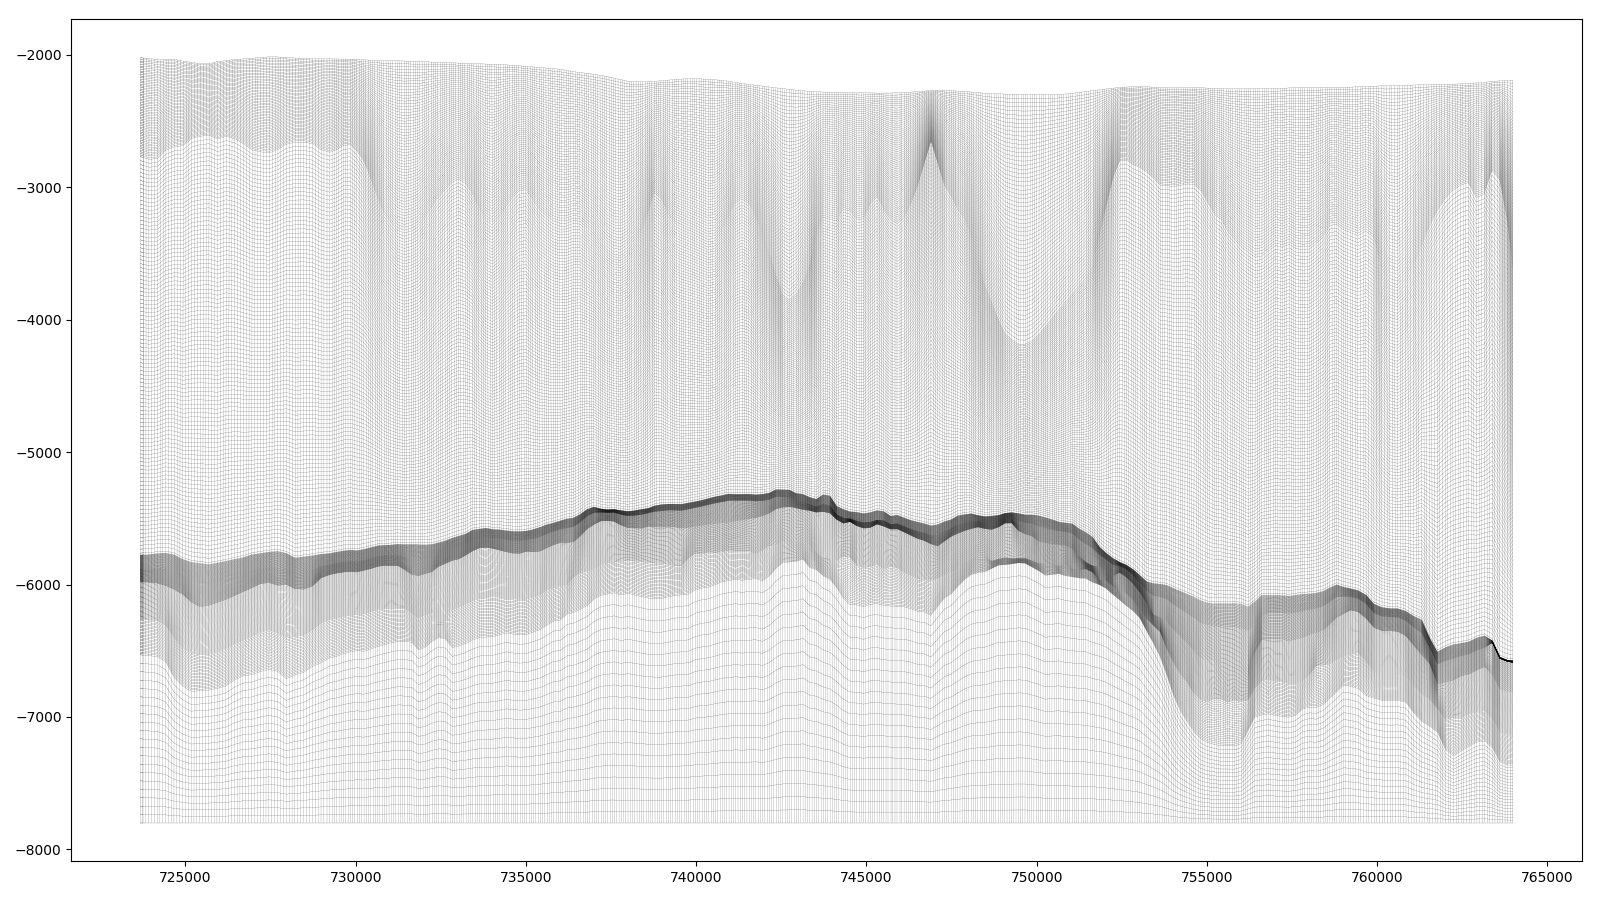
\includegraphics[width=\textwidth]{append/figs/93MM_grid.png}}
\qquad
\subfigure[ ]{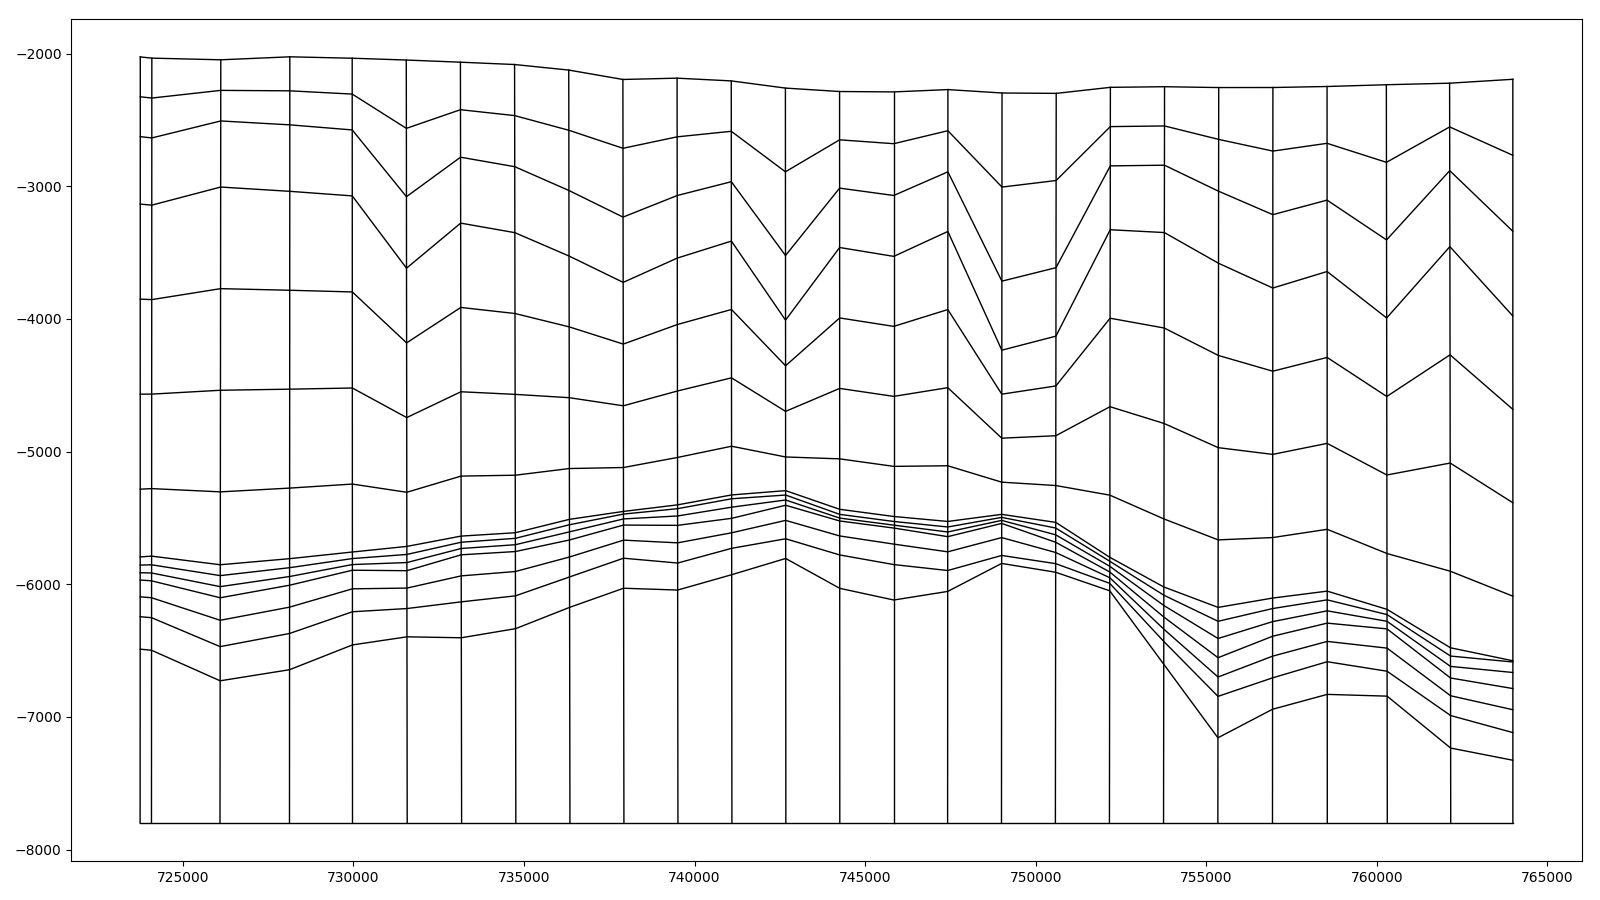
\includegraphics[width=\textwidth]{append/figs/93MM_24x24.png}}
\caption{Grid de simulação original (a) e após refinamento 24 x 24(b) para caso E } \label{fig:casoEgrid_figures}
\end{figure}
